\documentclass[10pt]{article}
\usepackage[a4paper, margin=1in]{geometry}
\usepackage[utf8]{inputenc}
\usepackage[spanish]{babel}
\usepackage{caratula}
\usepackage{amsmath}
\usepackage{amssymb}
\usepackage{hyperref}
\usepackage{enumitem}
\usepackage{graphicx}
\usepackage{subcaption} % Para subfiguras

\hypersetup{
    colorlinks=true,
    linkcolor=blue,
    filecolor=magenta,      
    urlcolor=cyan,
    pdftitle={Overleaf Example},
    pdfpagemode=FullScreen,
	}

\begin{document}

	\titulo{TP2}

	\fecha{\today}

	\materia{Introducción a la Investigación Operativa y Optimización}

	\integrante{Laks, Joaquín}{425/22}{laksjoaquin@gmail.com}
	\integrante{Szabo, Jorge}{1683/21}{jorgecszabo@gmail.com}
	\integrante{Wilders Azara, Santiago}{350/19}{santiago199913@gmail.com}

	\maketitle

\section{Introducción}

En este trabajo práctico abordamos el problema de distribución de productos a clientes con metodologías distintas, variaciones del problema del viajante, incorporando repartidores a pie o en bicicleta y productos refrigerados. En particular para estas metodologías, se busca identificar qué clientes deben ser visitados directamente por el camión y cuáles pueden ser atendidos por repartidores a pie/bicicleta desde determinadas paradas del camión, respetando restricciones operativas como la distancia máxima de reparto o la entrega de productos refrigerados.

El objetivo principal es modelar, generar instancias y analizar los resultados obtenidos para las distintas metodologías comparando sus costos. Además, se analizarán los tiempos de cómputo requeridos utilizando diferentes alternativas algorítmicas mediante los parámetros que provee CPLEX.

A continuación, se describen las distintas metodologías de reparto consideradas y los modelos propuestos para representarlas.
\section{Modelos}


\subsection{Modelo para la metodología actual (TSP)}

La metodología actual consiste en que el camión visita a cada cliente y entrega sus pedidos, es decir, idéntica al problema del viajante clásico. Usamos el modelo de Miller, Tucker, y Zemlin para simularlo y como base para las otras metodologías.

\subsection{Modelo con repartidores (MR)}

Se desea evaluar una nueva metodología de distribución en la cual el camión realiza paradas en ciertos clientes, y desde esas paradas se pueden realizar entregas adicionales mediante repartidores a pie o en bicicleta, siempre que los clientes estén a una distancia menor o igual a $dist\_max$. Cada repartidor tiene un costo por cliente atendido, y esta restringido a una única entrega en caso de que sea un producto refrigerado.


Basado en el modelo anterior, agregamos variables para distinguir cuándo un cliente fue visitado por repartidor a bicicleta y cuándo fue visitado por el camión.

	\vspace{5mm}

	Dado un cliente $i$, definimos $D_i$ como el conjunto de clientes a una distancia menor a \texttt{dist\_max} de $i$.
	
	\begin{align*}
		x_{ij} &= 
		\begin{cases}
			1 & \text{si el camión se mueve desde el cliente $v_i$ al cliente $v_j$} \\
			0 & \text{en caso contrario}
		\end{cases} \\[1em]
		u_i &= \text{posición del cliente $i$ en el circuito del camión (irrelevante si no es visitado)} \\[1em]
		b_{ij} &= 
		\begin{cases}
			1 & \text{si se envió un repartidor desde $v_i$ hasta $v_j$} \\
			0 & \text{en caso contrario}
		\end{cases} \\[1em]
		r_i &=
		\begin{cases}
			1 & \text{si al cliente $v_i$ se le entrega un producto que necesita refrigeración} \\
			0 & \text{en caso contrario}
		\end{cases}
	\end{align*}
	
\vspace{5mm}

	Entonces con $n = cant\_clientes$, buscamos:

	\[
		\text{Min} \sum_{\substack{v_i, v_j \in V \\ i \neq j}} c_{ij} x_{ij} 
		+ costo\_repartidor\, b_{ij}
		\]
\vspace{30mm}

	s.a.

	\[
	\begin{array}{l l l}
		\sum_{j \neq i} x_{ji} + \sum_{j \neq i} b_{ji} = 1 & \forall v_i \in V & \text{\scriptsize (a toda ciudad se entra una vez, por camión o bicicleta)} \\
		\\
		\sum_{j \neq i} x_{ij} = \sum_{j\neq i} x_{ji} & \forall v_i \in V & \text{\scriptsize (si se entró en camión, se sale por camión)} \\
		\\
		M(1 - \sum_{j \neq i} b_{ji}) \geq \sum_{j \neq i} b_{ij} + \sum_{j \neq i} x_{ij} & \forall v_i \in V, M \geq |V| & \text{\scriptsize (si se entra en bicicleta, no se sale de ninguna forma)} \\
		\\
		\sum_{j \in D_i} b_{ij} r_j \leq 1 & \forall v_i \in V & \text{\scriptsize (ningún repartidor tiene más de un refrigerado)} \\
		\\
		u_i - u_j + (n - 1) x_{ij} \leq n - 2 & \forall v_i \neq v_j \in V - \{v_1\} & \text{\scriptsize (continuidad)} \\
		\\
		u_1 = 0, 1 \leq u_i \leq n-1 & \forall v_i \in V - \{v_1\} \\
		\\
		x_{ij}, b_{ij} \in \{0,1\}, u_i \in \mathbb{Z}_{\geq 0}
	\end{array}
	\]
	
	
	
	\subsection{Modelos con restricciones agregadas (MR4 y MRE)}
	
	Estos metodologías extienden la anterior incorporando una nueva restricción adicional en cada caso:
	
	\begin{description}
		\item[MR4:] Si se contrata un repartidor en una parada de camión determinada, este debe realizar al menos cuatro entregas.
		\item[MRE:] Hay un conjunto de clientes $E$ que deben ser visitados exclusivamente por un camión. Es decir, sus paquetes no pueden ser repartidos por un repartidor en bicicleta.
	\end{description}
	
	Entonces, para cada modelo se extiende el presentado en la sección anterior con su respectiva nueva restricción:
	
	\begin{description}
		\item[MR4:]
		\[
		4(1 - b_{ij}) + \sum_{v_k \in D_i} b_{ik} \geq 4 \quad \forall v_i, v_j \in V \times V
		\]
		
		\item[MRE:]
		\[
		\sum_{v_i \in V}  b_{ij} = 0 \quad \forall v_j \in E
		\]
	\end{description}
	
	No hay cambios en las variables, función objetivo o las demás restricciones.


	\section{Experimentación}

	Usamos un generador de instancias aleatorias para generar mapas donde algunos caminos son posibles y otros no, asignando distanias y costos al azar, así como también qué clientes necesitan refrigeración o tienen que vistiarse con camión en el último modelo. También sacamos datos de posiciones de ciudades de \url{https://people.sc.fsu.edu/~jburkardt/datasets/cities/cities.html}, usamos las distancias y las modificamos aleatoriamente para crear una instancia con costos proporcionales. De esta página tomamos las instancias \texttt{wg59} con 59 ciudades de Alemania Oriental, y \texttt{qa194} con 194 ciudades de Catar. Nos interesó crear instancias con información geográfica para tener una distribución orgánica de los puntos, \texttt{qa194} en particular, además de ser una instancia grande, es interesante porque la densidad de los puntos es muy poco uniforme.

	Para decidir si un viaje entre dos puntos es posible agregamos aleatoriamente aristas entre los puntos, llamamos \textit{ralas} a las instancias donde la probabilidad de agregar una arista es de $0.3$ y \textit{densas} cuando la probabilidad es de $0.9$. Siempre asegurándonos de que el grafo resultante quede conexo.

	También con los puntos creamos instancias donde la proporción de refrigerados es del $70\%$ y otras donde es el $10\%$. Hicimos lo mismo con los exclusivos.

	Por último también agregamos instancias donde la distancia máxima del repartidor era muy corta o muy larga, y donde el repartidor era muy barato o muy caro. Por defecto la distancia máxima del repartidor la tomamos como la mediana de todas las distancias, pero para representar una distancia máxima más corta usamos el primer quintil, y para una más larga el tercero. Hicimos lo mismo con los costos para representar cuándo el repartidor es más caro o más barato.


\section{Análisis de sensibilidad de los parámetros del modelo}


\section{Comparación de costos entre metodologías}
Para analizar el rendimiento de las distintas metodologías, definimos y generamos dos tipos distintos de instancias, uno con clientes uniformemente distribuidos y el otro conformado por varios clusters distintos donde se concentran grupos de clientes dentro de un radio. En las figuras~\ref{fig:compuesta1} y~\ref{fig:compuesta2} respectivamente, se puede apreciar la diferencia de los tipos.

\vspace{5mm}

\begin{figure}[htbp]
	\centering
	\begin{subfigure}[b]{0.45\textwidth}
		\centering
		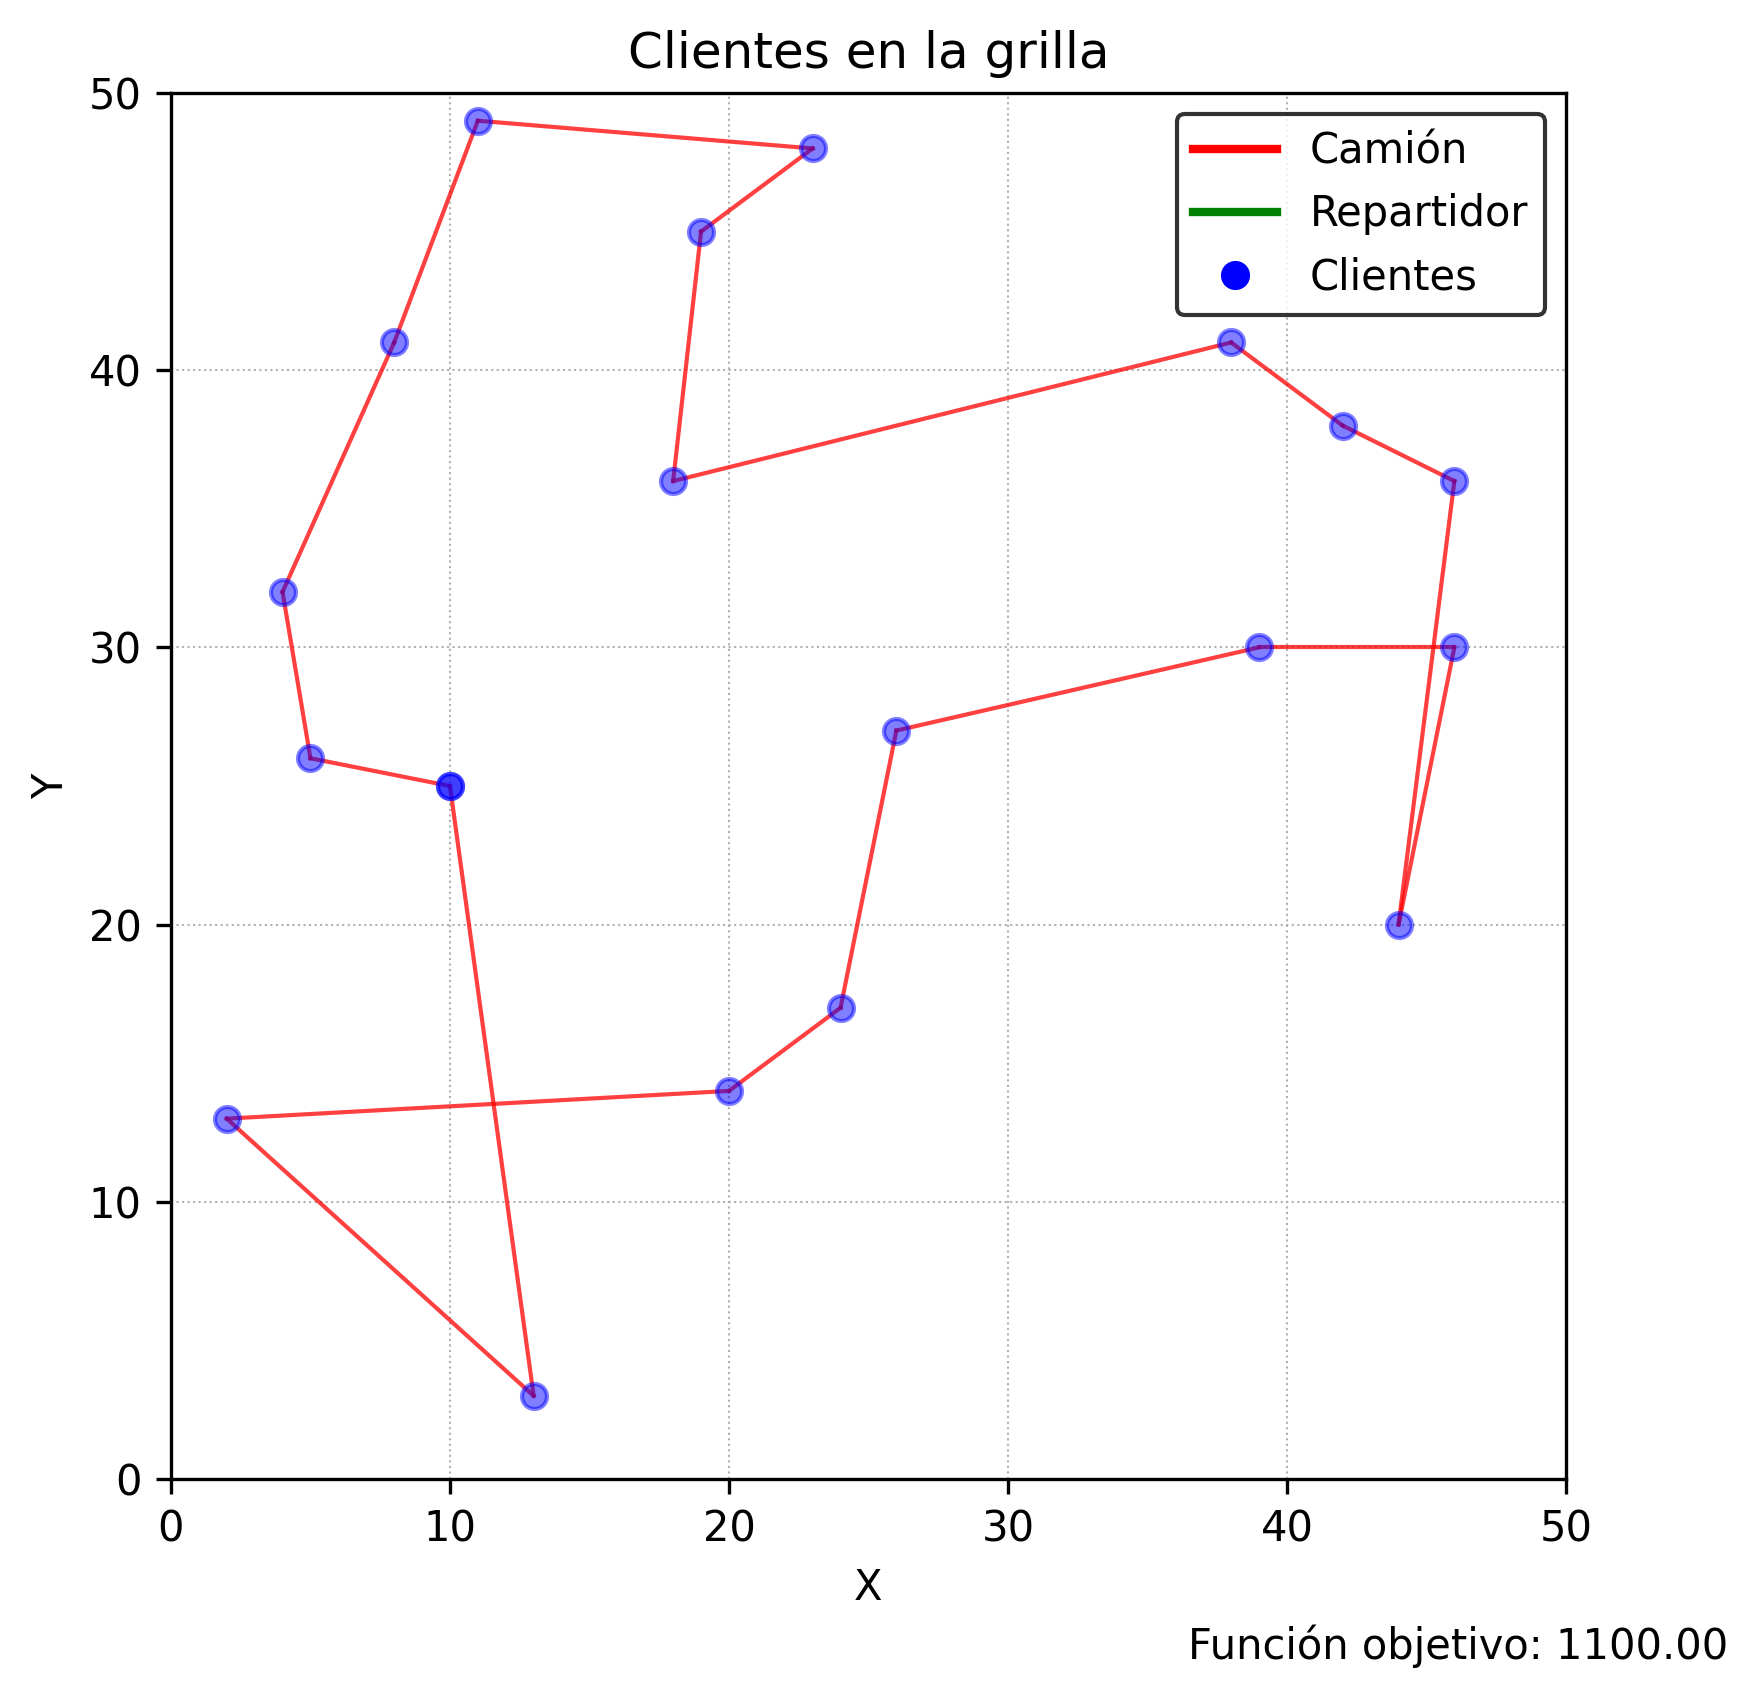
\includegraphics[width=\textwidth]{figuras/plano_uniforme_tsp_2.png}
		\caption{Metodología actual (TSP)}
		\label{fig:sub1}
	\end{subfigure}
	\hfill
	\begin{subfigure}[b]{0.45\textwidth}
		\centering
		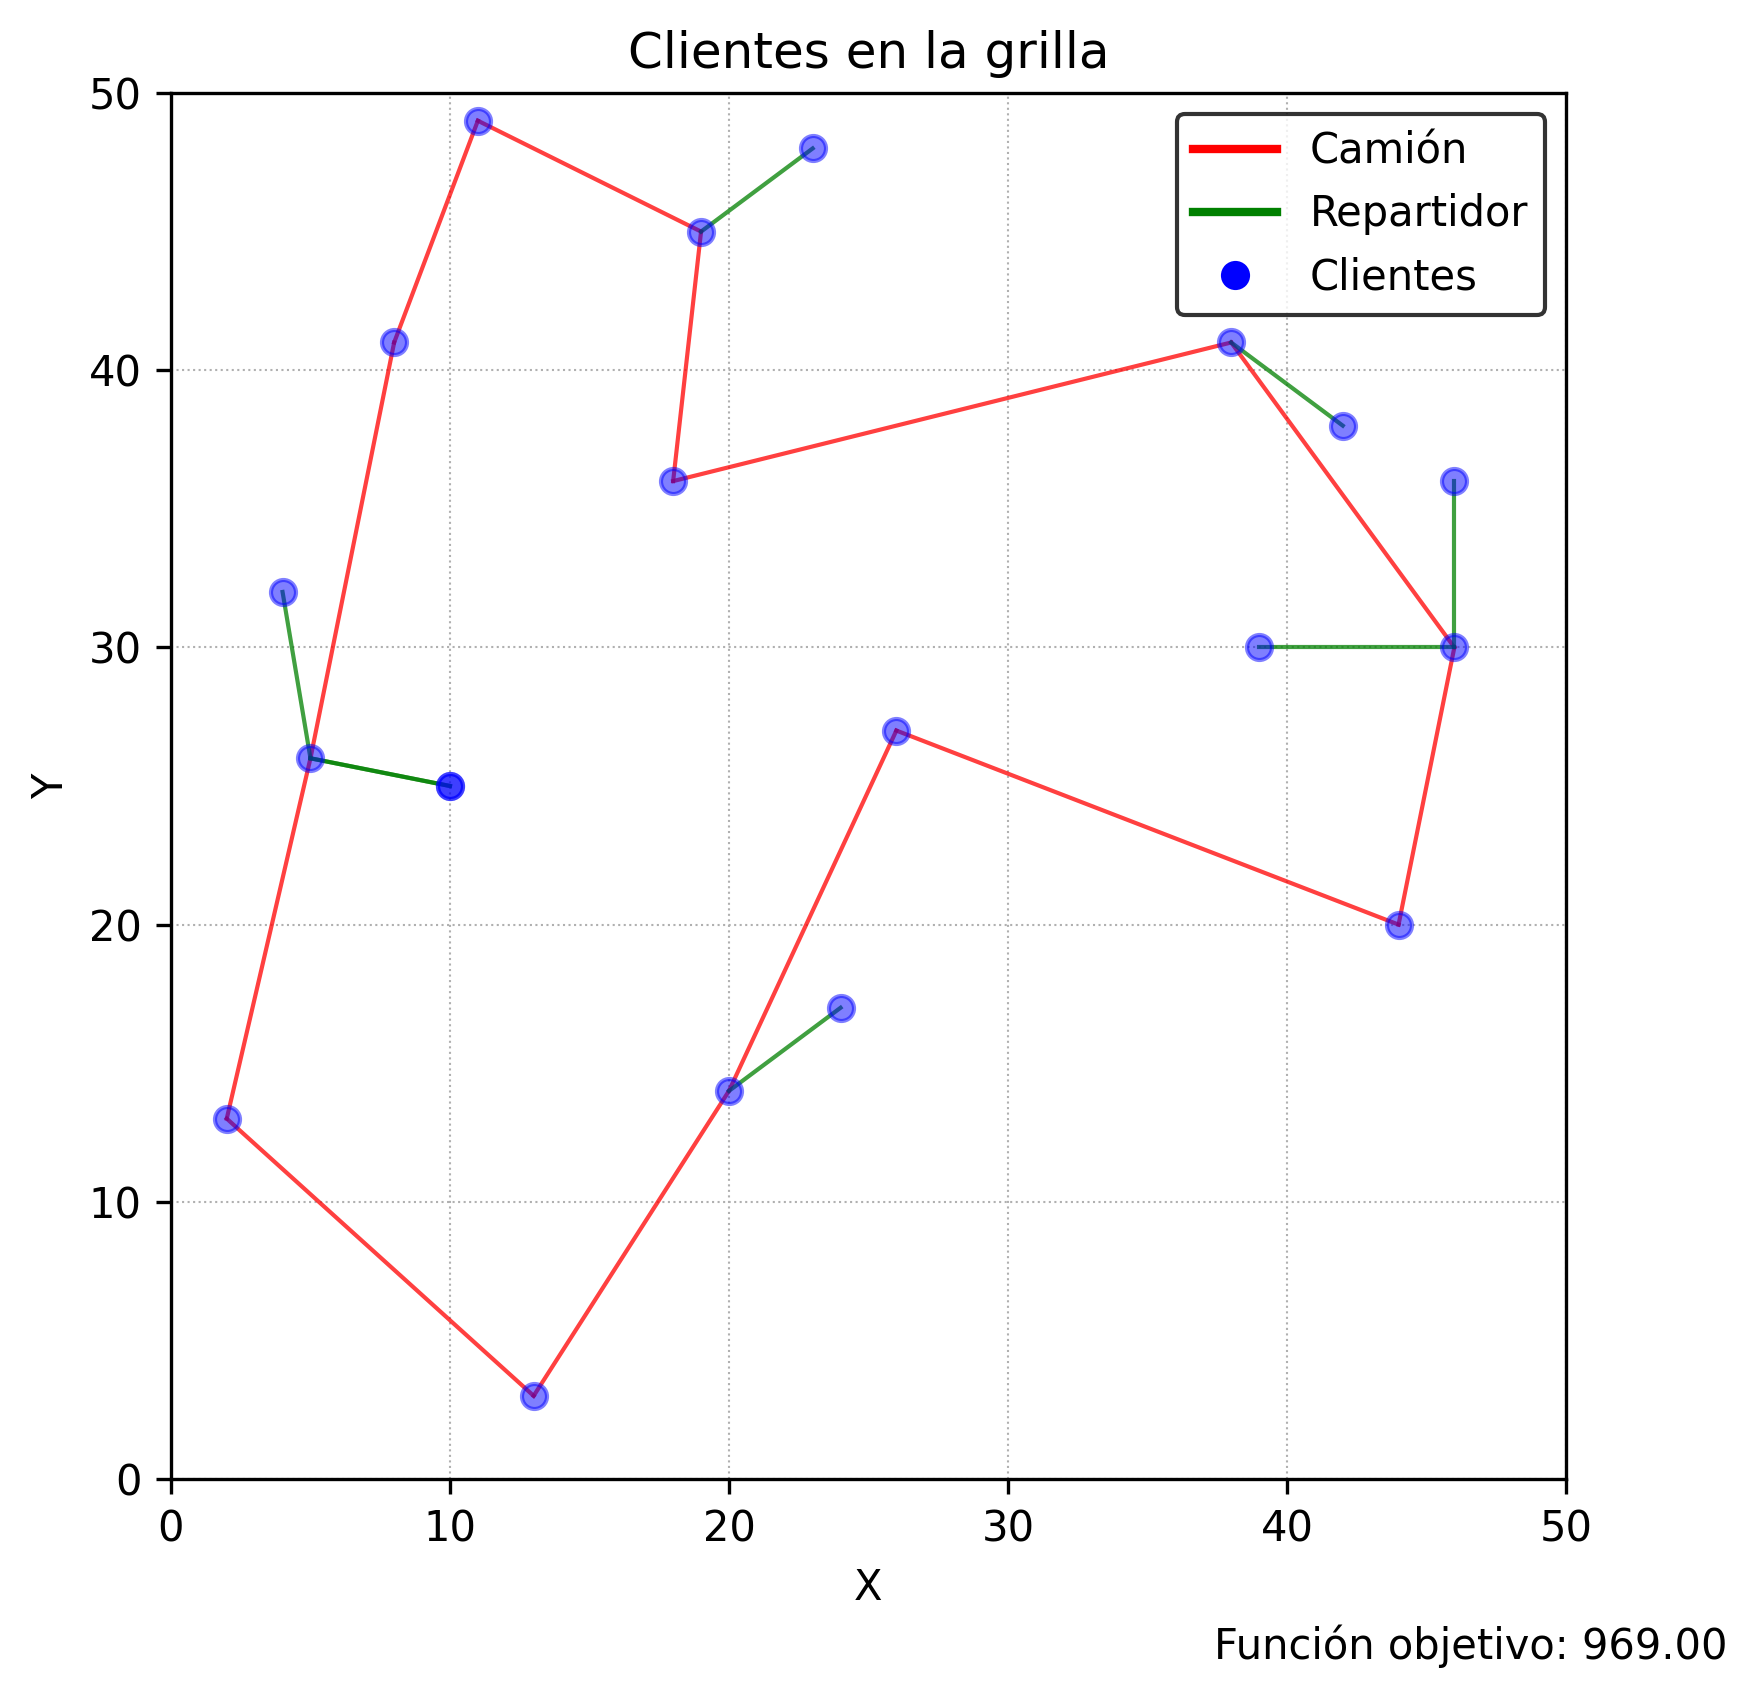
\includegraphics[width=\textwidth]{figuras/plano_uniforme_repartidores_2.png}
		\caption{Metodología con repartidores (MR)}
		\label{fig:sub2}
	\end{subfigure}
	
	\vspace{0.5cm}
	
	\begin{subfigure}[b]{0.45\textwidth}
		\centering
		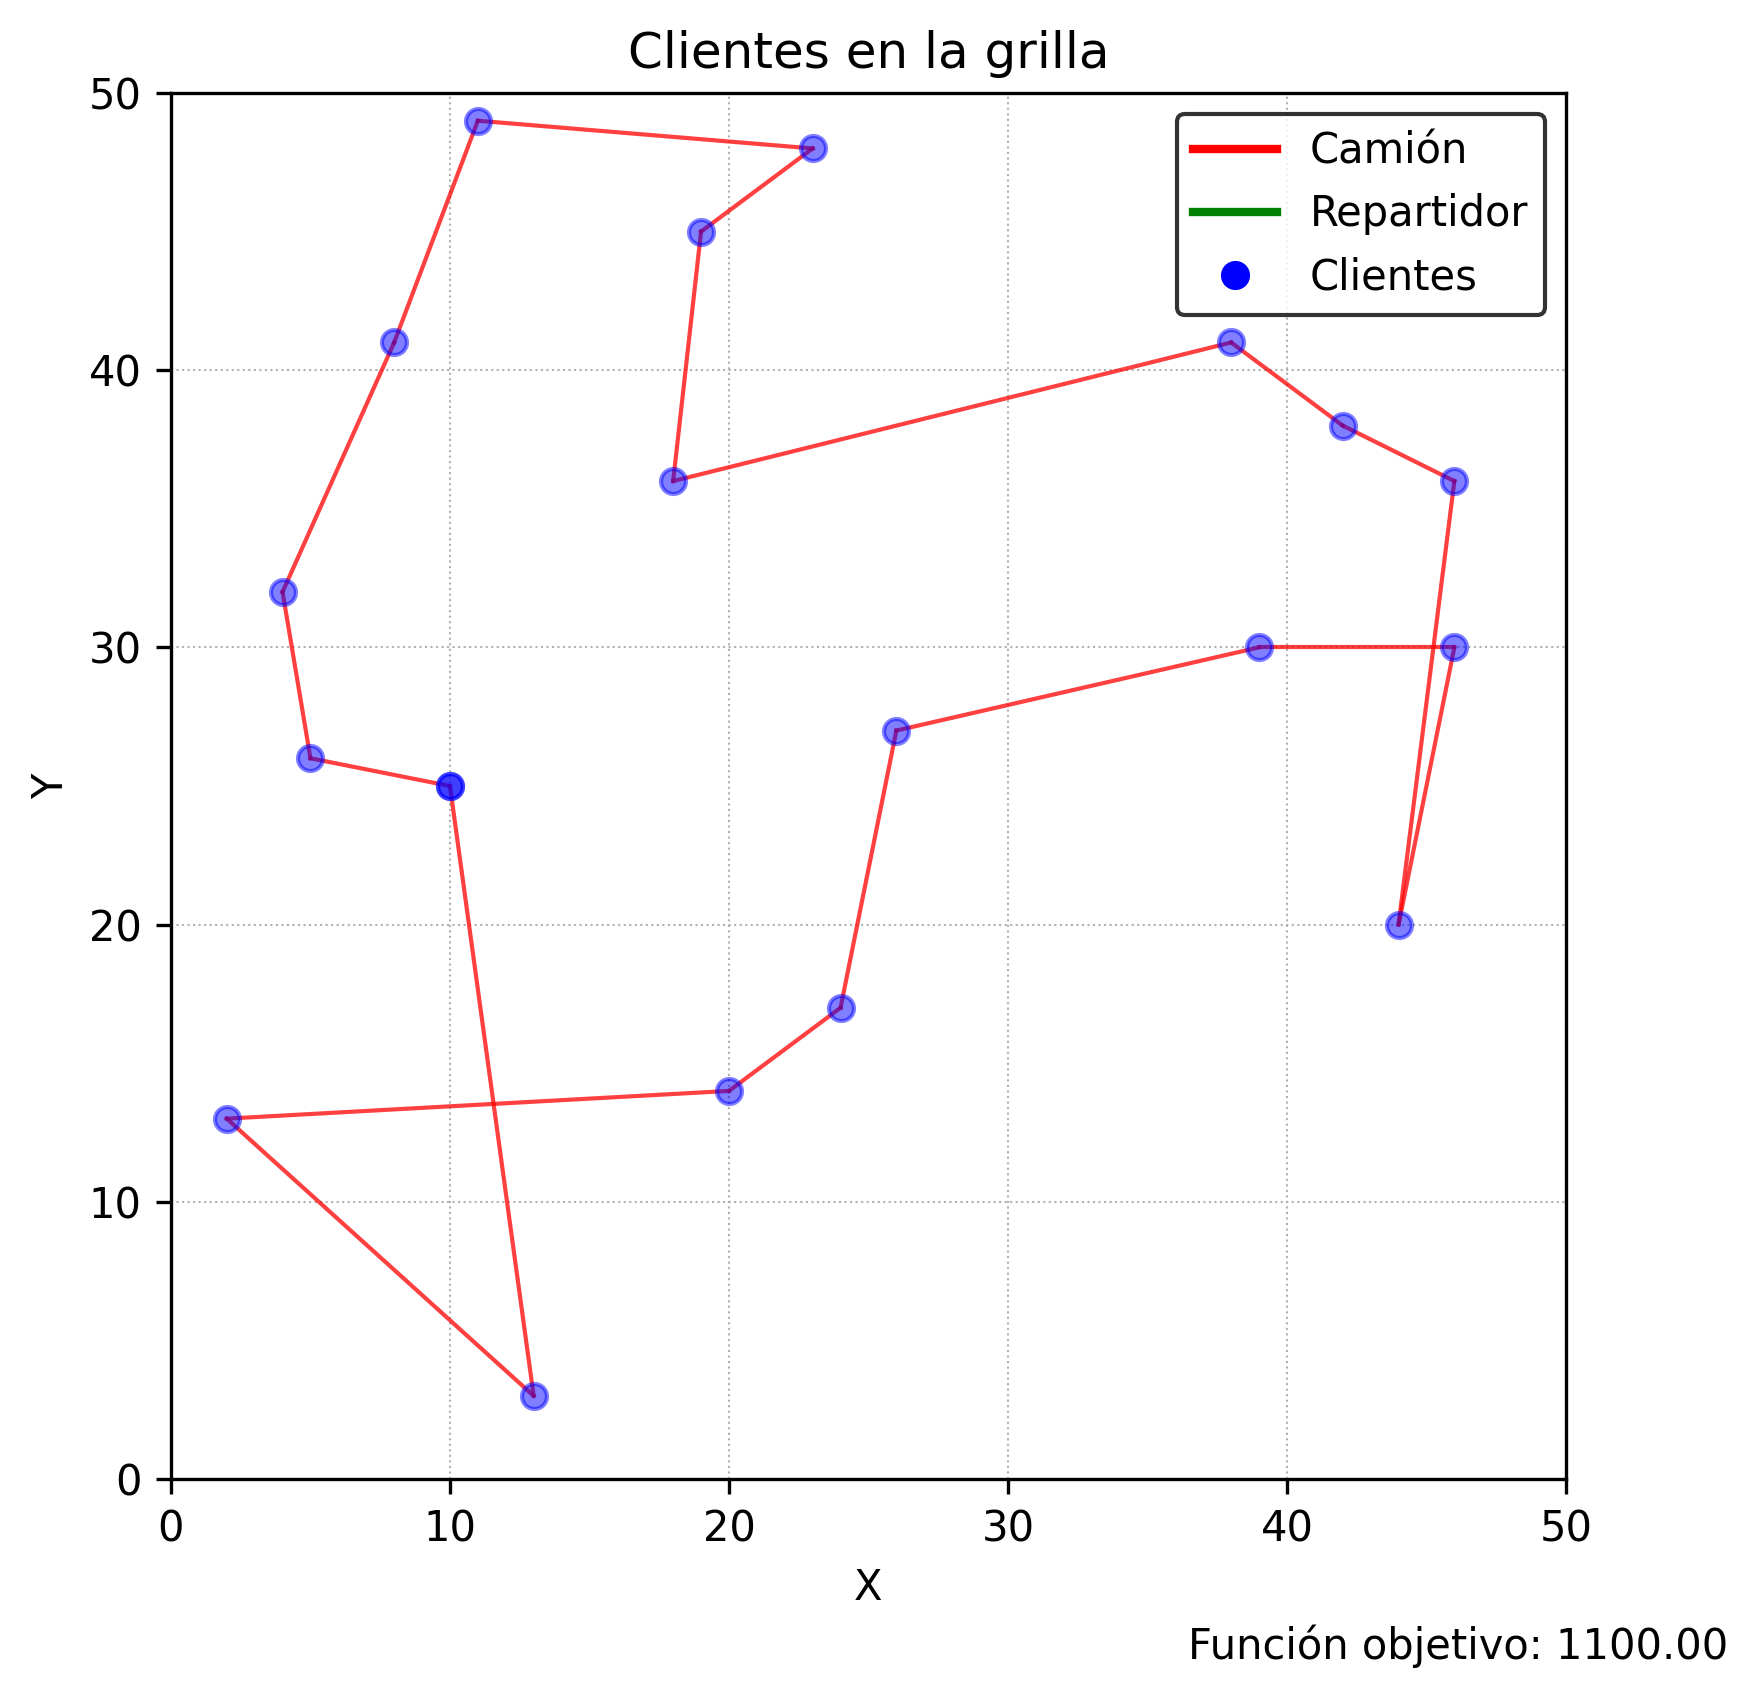
\includegraphics[width=\textwidth]{figuras/plano_uniforme_cuatro_o_mas_2.png}
		\caption{Metodología con repartidores de al menos cuatro entregas (MR4)}
		\label{fig:sub3}
	\end{subfigure}
	\hfill
	\begin{subfigure}[b]{0.45\textwidth}
		\centering
		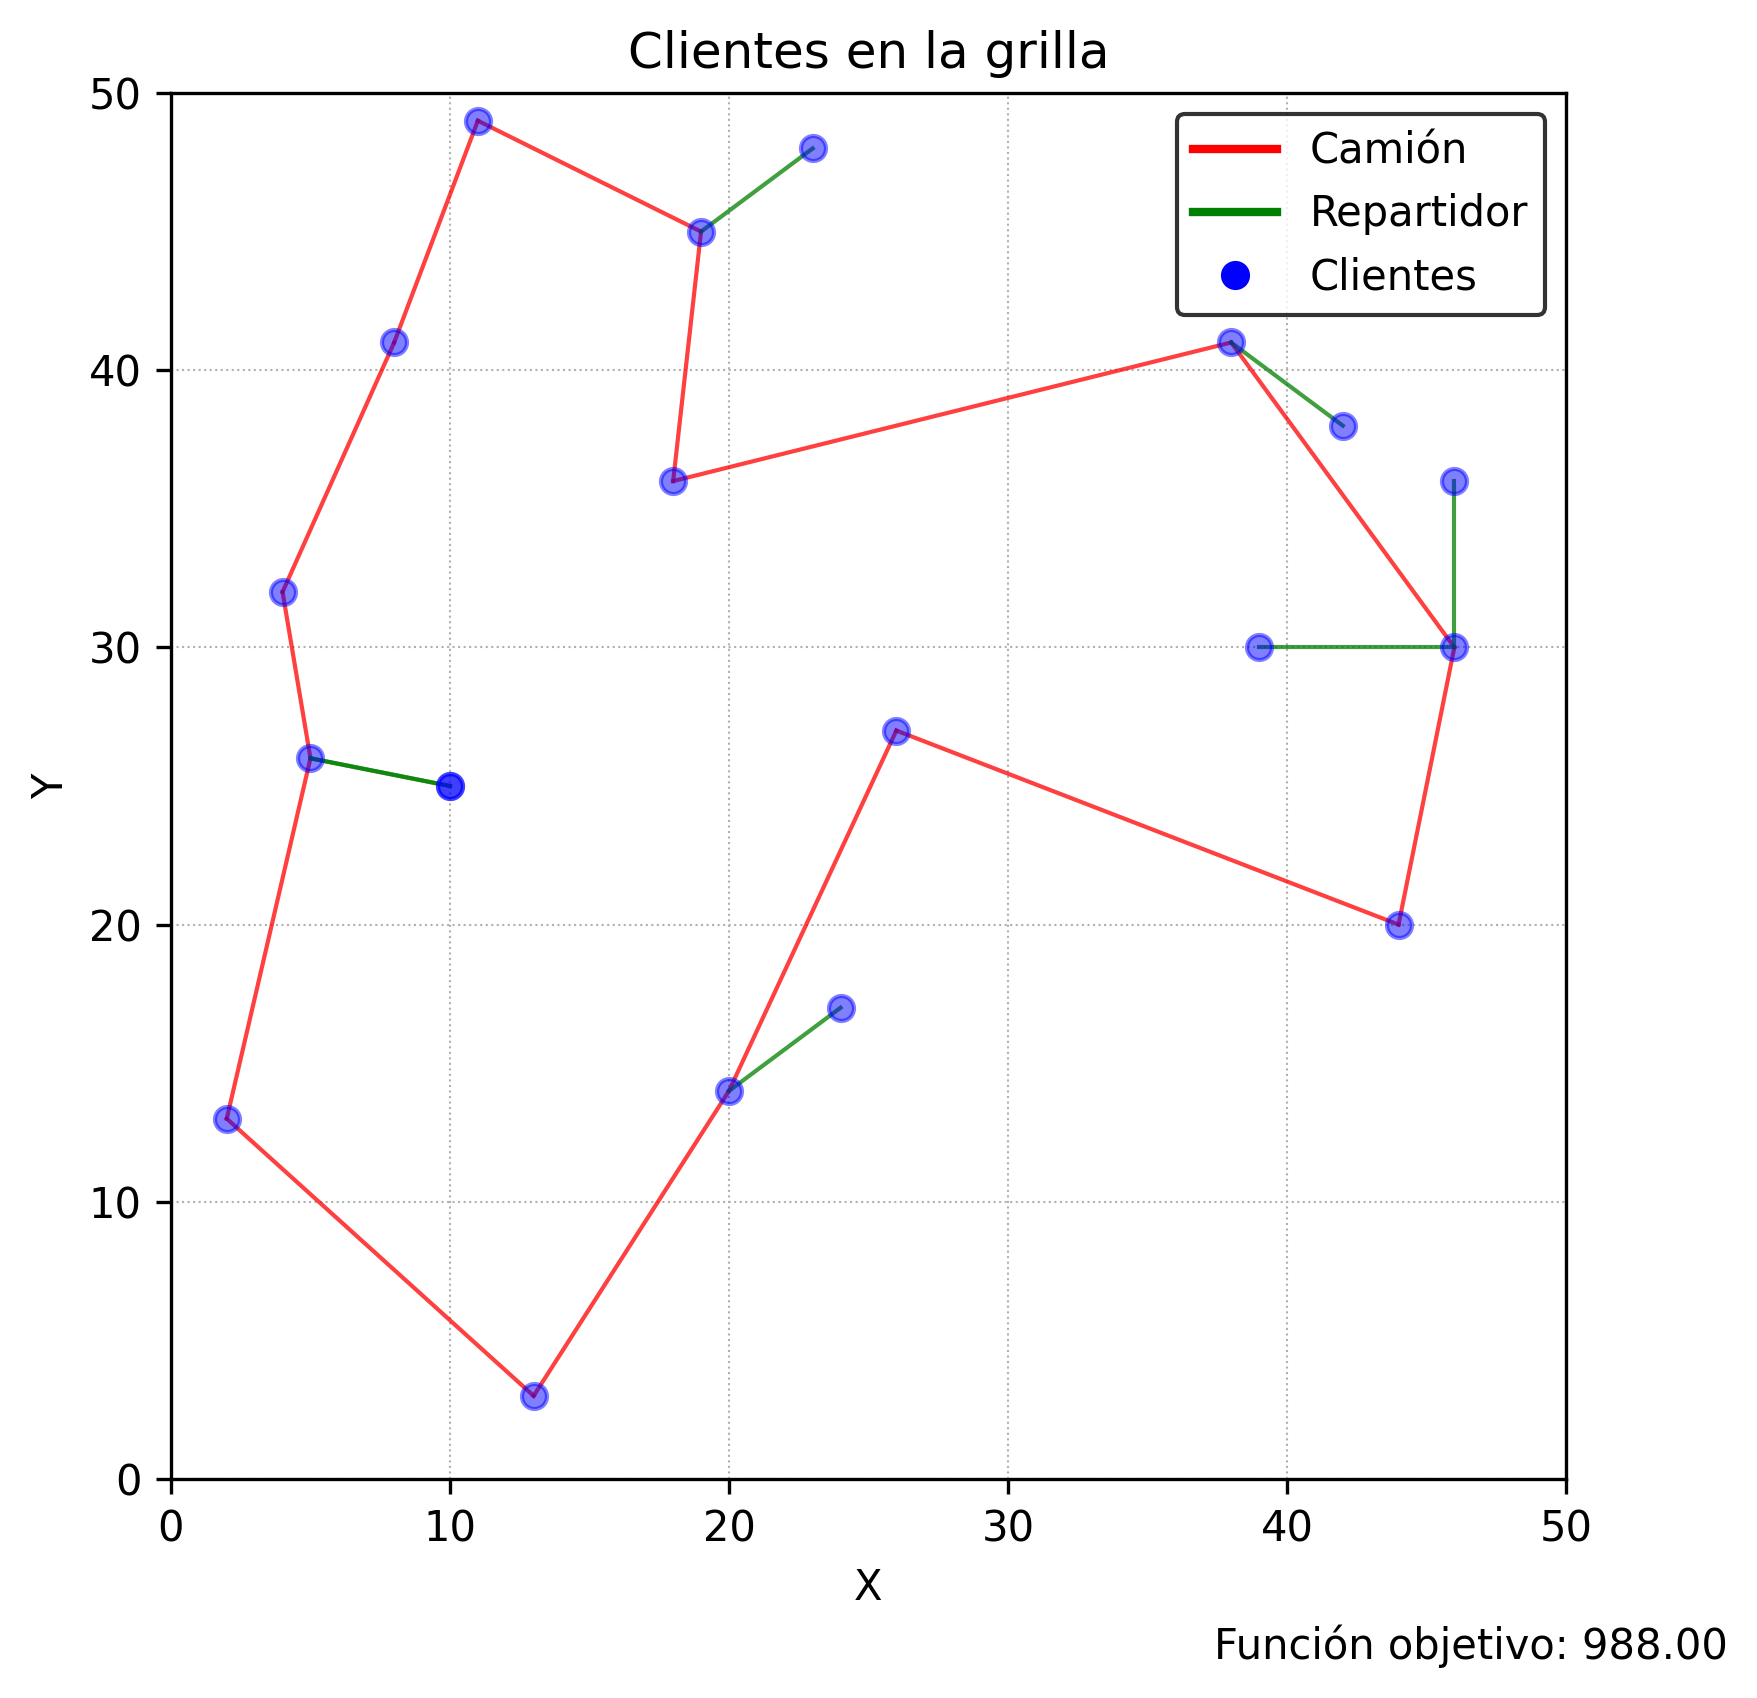
\includegraphics[width=\textwidth]{figuras/plano_uniforme_exclusivos_2.png}
		\caption{Metodología con clientes exclusivos (MRE)}
		\label{fig:sub4}
	\end{subfigure}
	
	\caption{Optimización de una misma instancia \textbf{uniformemente distribuida} con los distintos modelos.}
	\label{fig:compuesta1}
\end{figure}

\clearpage

\begin{figure}[htbp]
	\centering
	\begin{subfigure}[b]{0.45\textwidth}
		\centering
		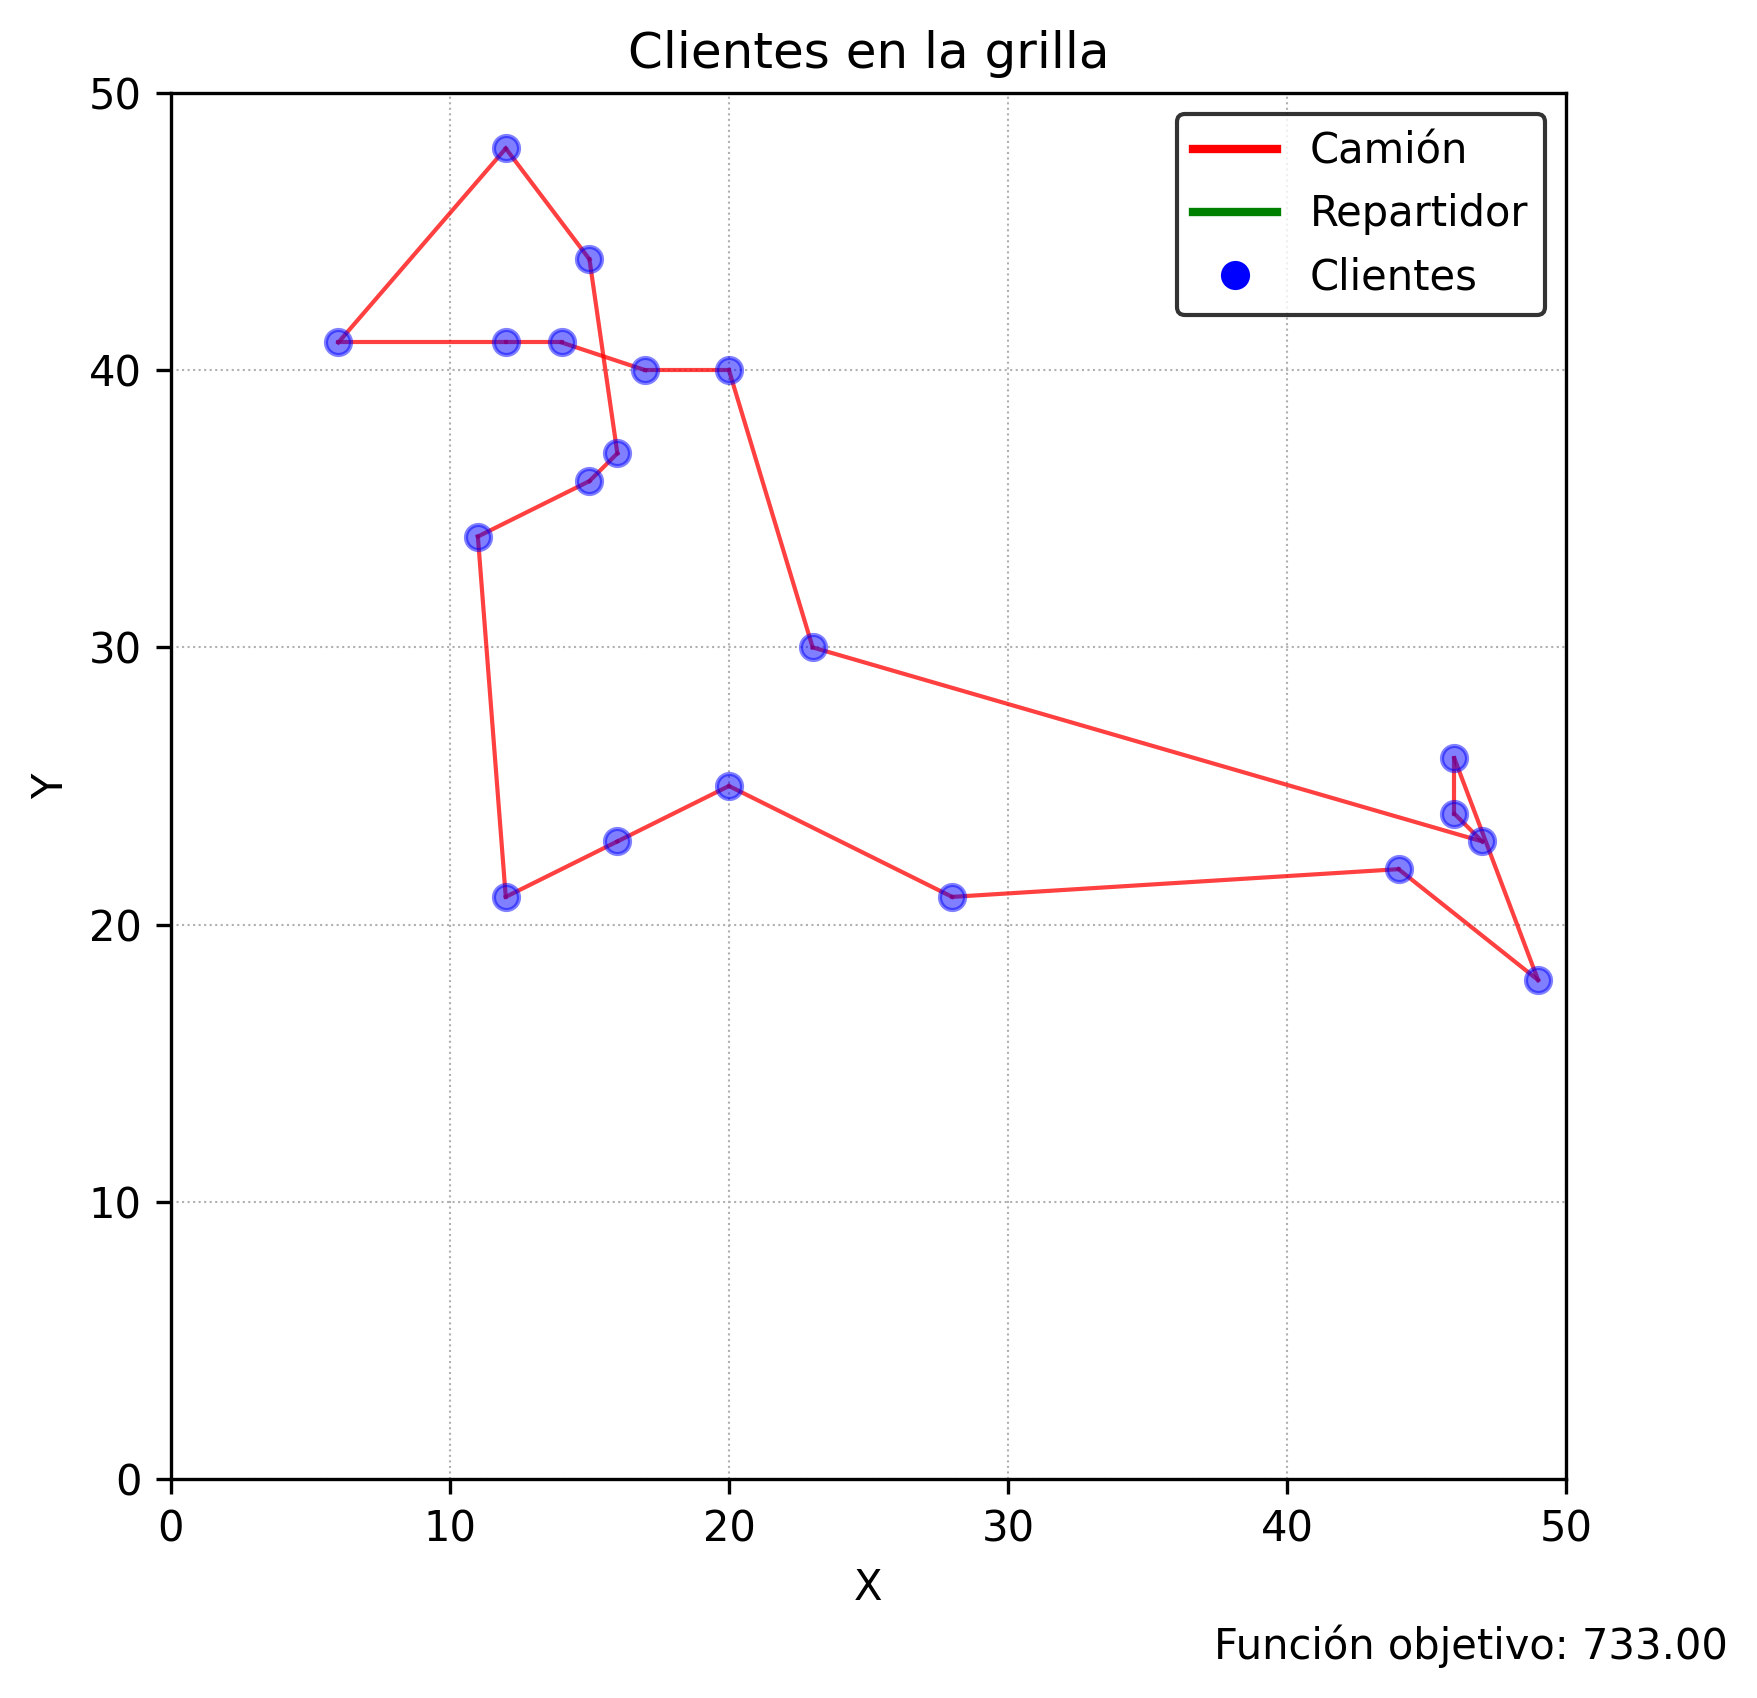
\includegraphics[width=\textwidth]{figuras/plano_clusters_tsp_0.png}
		\caption{Metodología actual (TSP)}
		\label{fig:sub1}
	\end{subfigure}
	\hfill
	\begin{subfigure}[b]{0.45\textwidth}
		\centering
		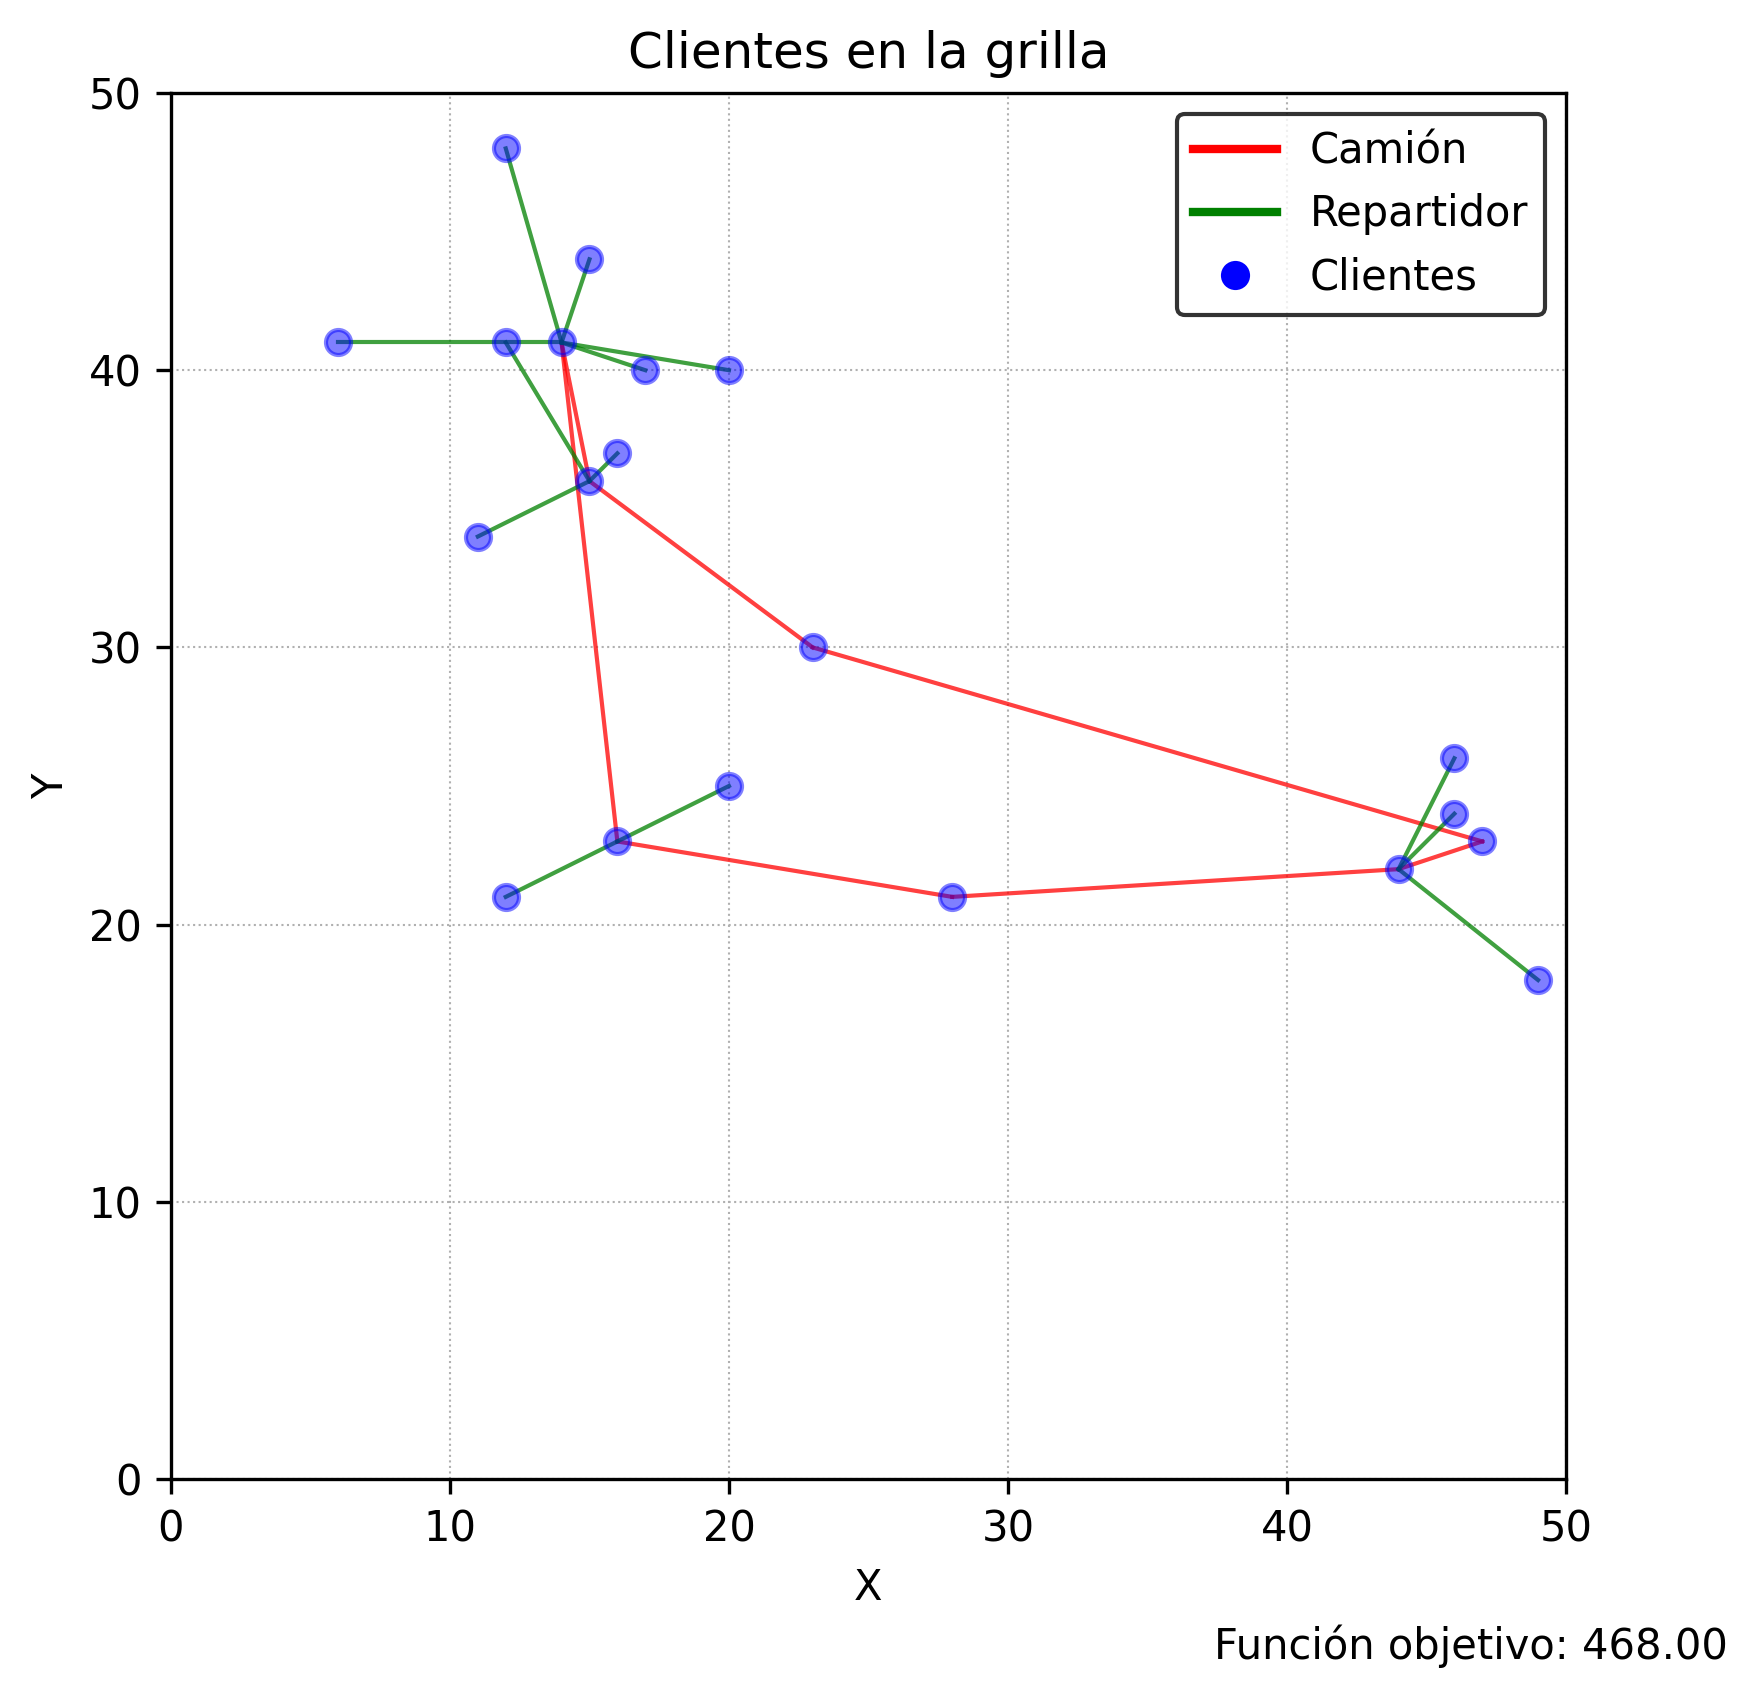
\includegraphics[width=\textwidth]{figuras/plano_clusters_repartidores_0.png}
		\caption{Metodología con repartidores (MR)}
		\label{fig:sub2}
	\end{subfigure}
	
	\vspace{0.5cm}
	
	\begin{subfigure}[b]{0.45\textwidth}
		\centering
		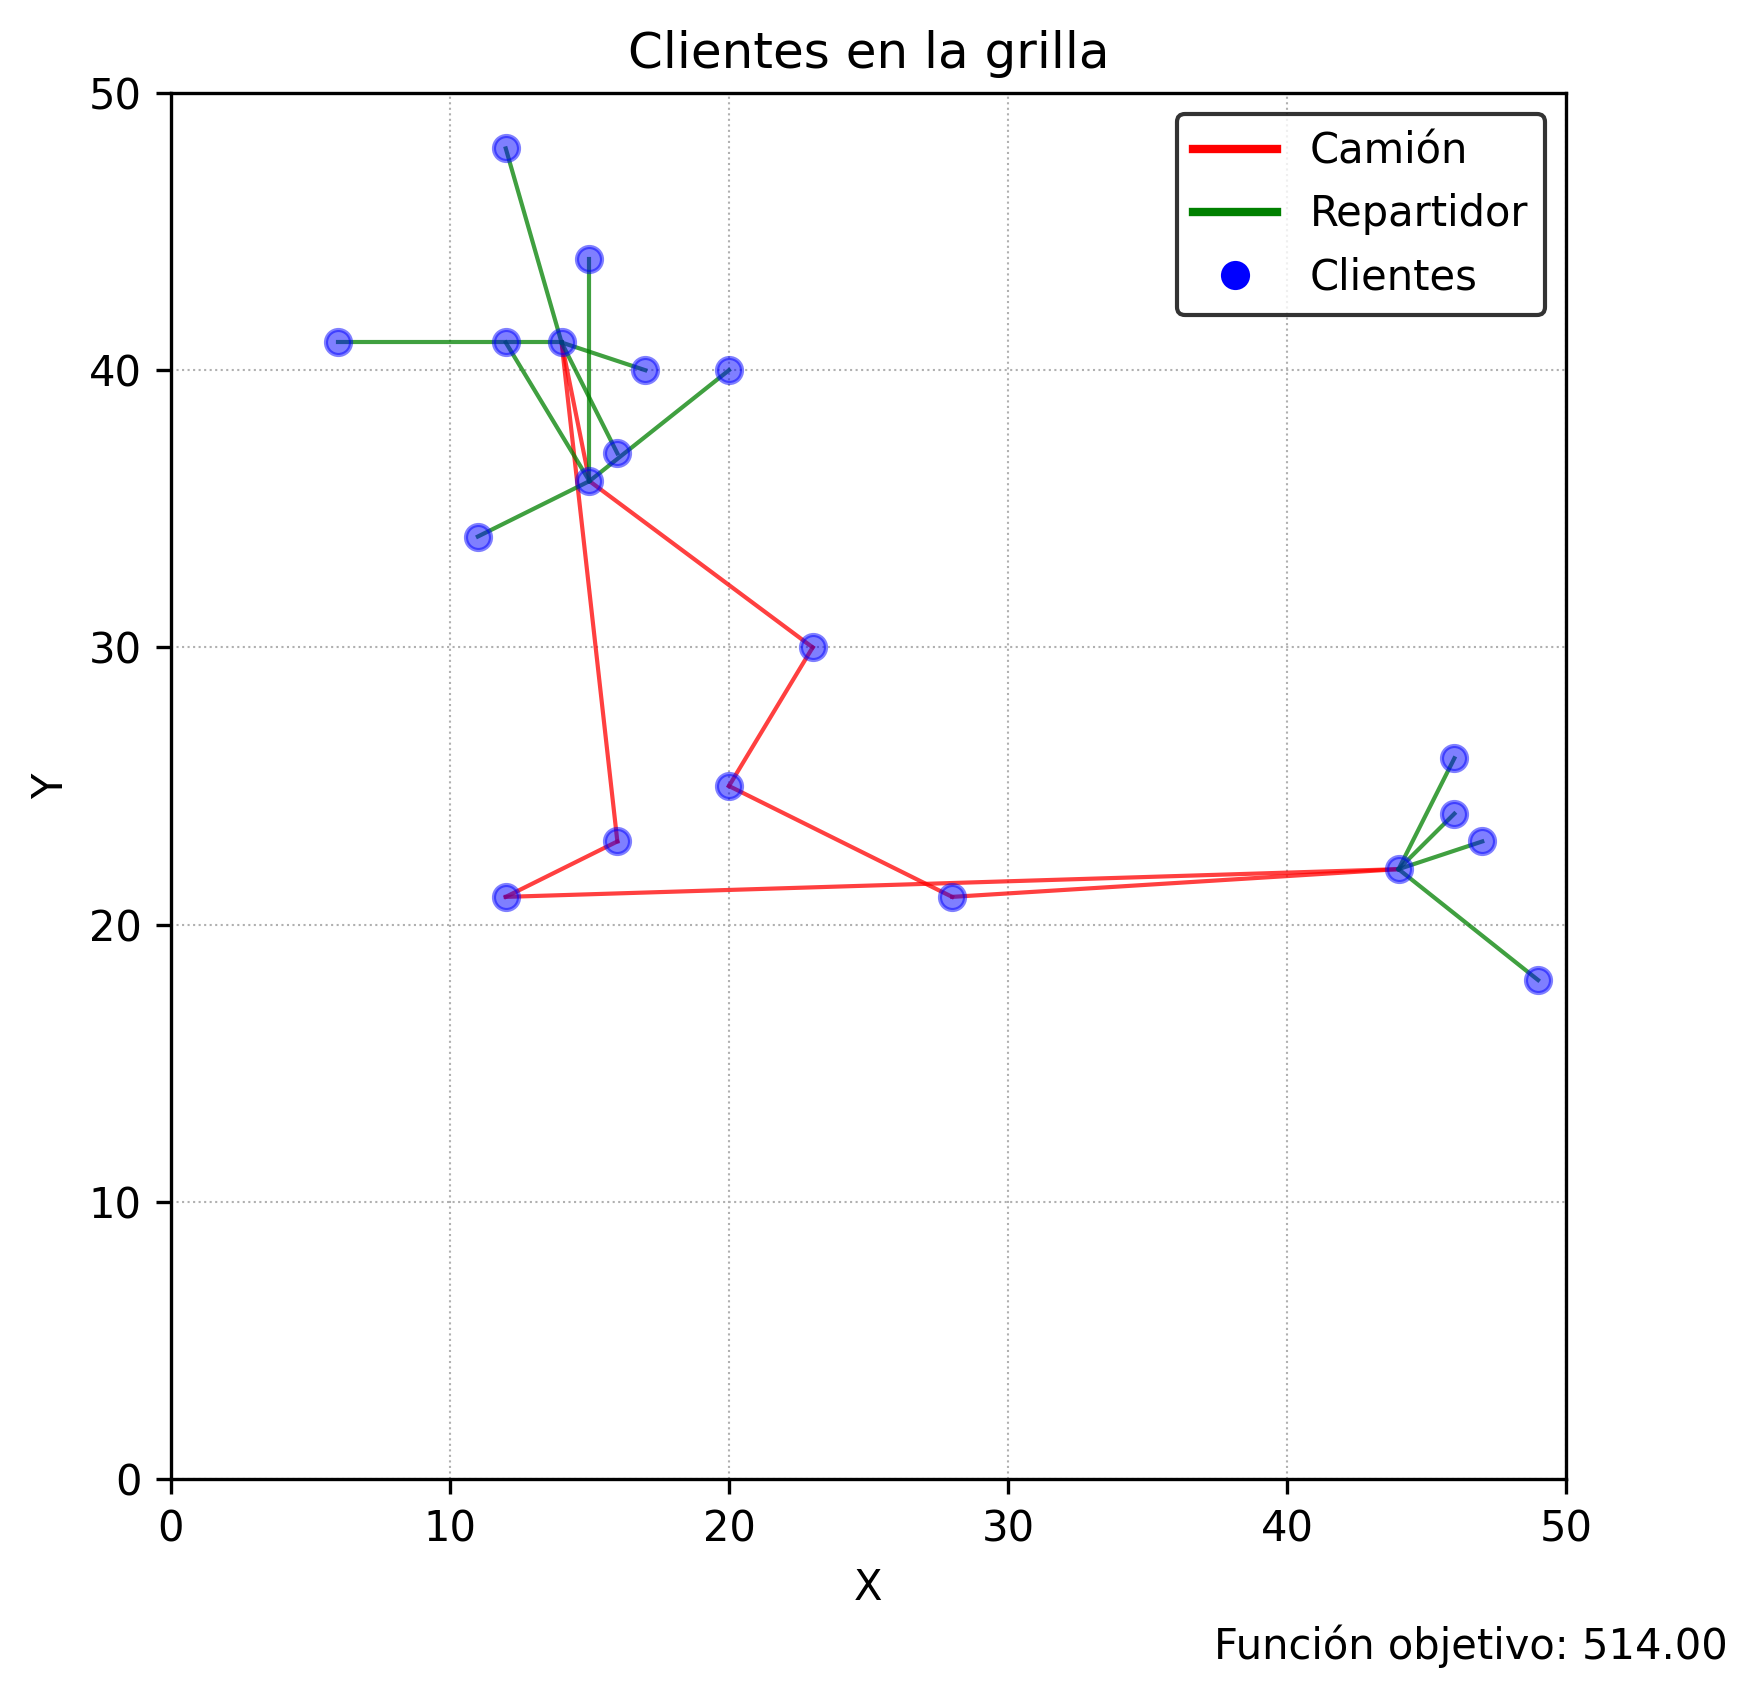
\includegraphics[width=\textwidth]{figuras/plano_clusters_cuatro_o_mas_0.png}
		\caption{Metodología con repartidores de al menos cuatro entregas (MR4)}
		\label{fig:sub3}
	\end{subfigure}
	\hfill
	\begin{subfigure}[b]{0.45\textwidth}
		\centering
		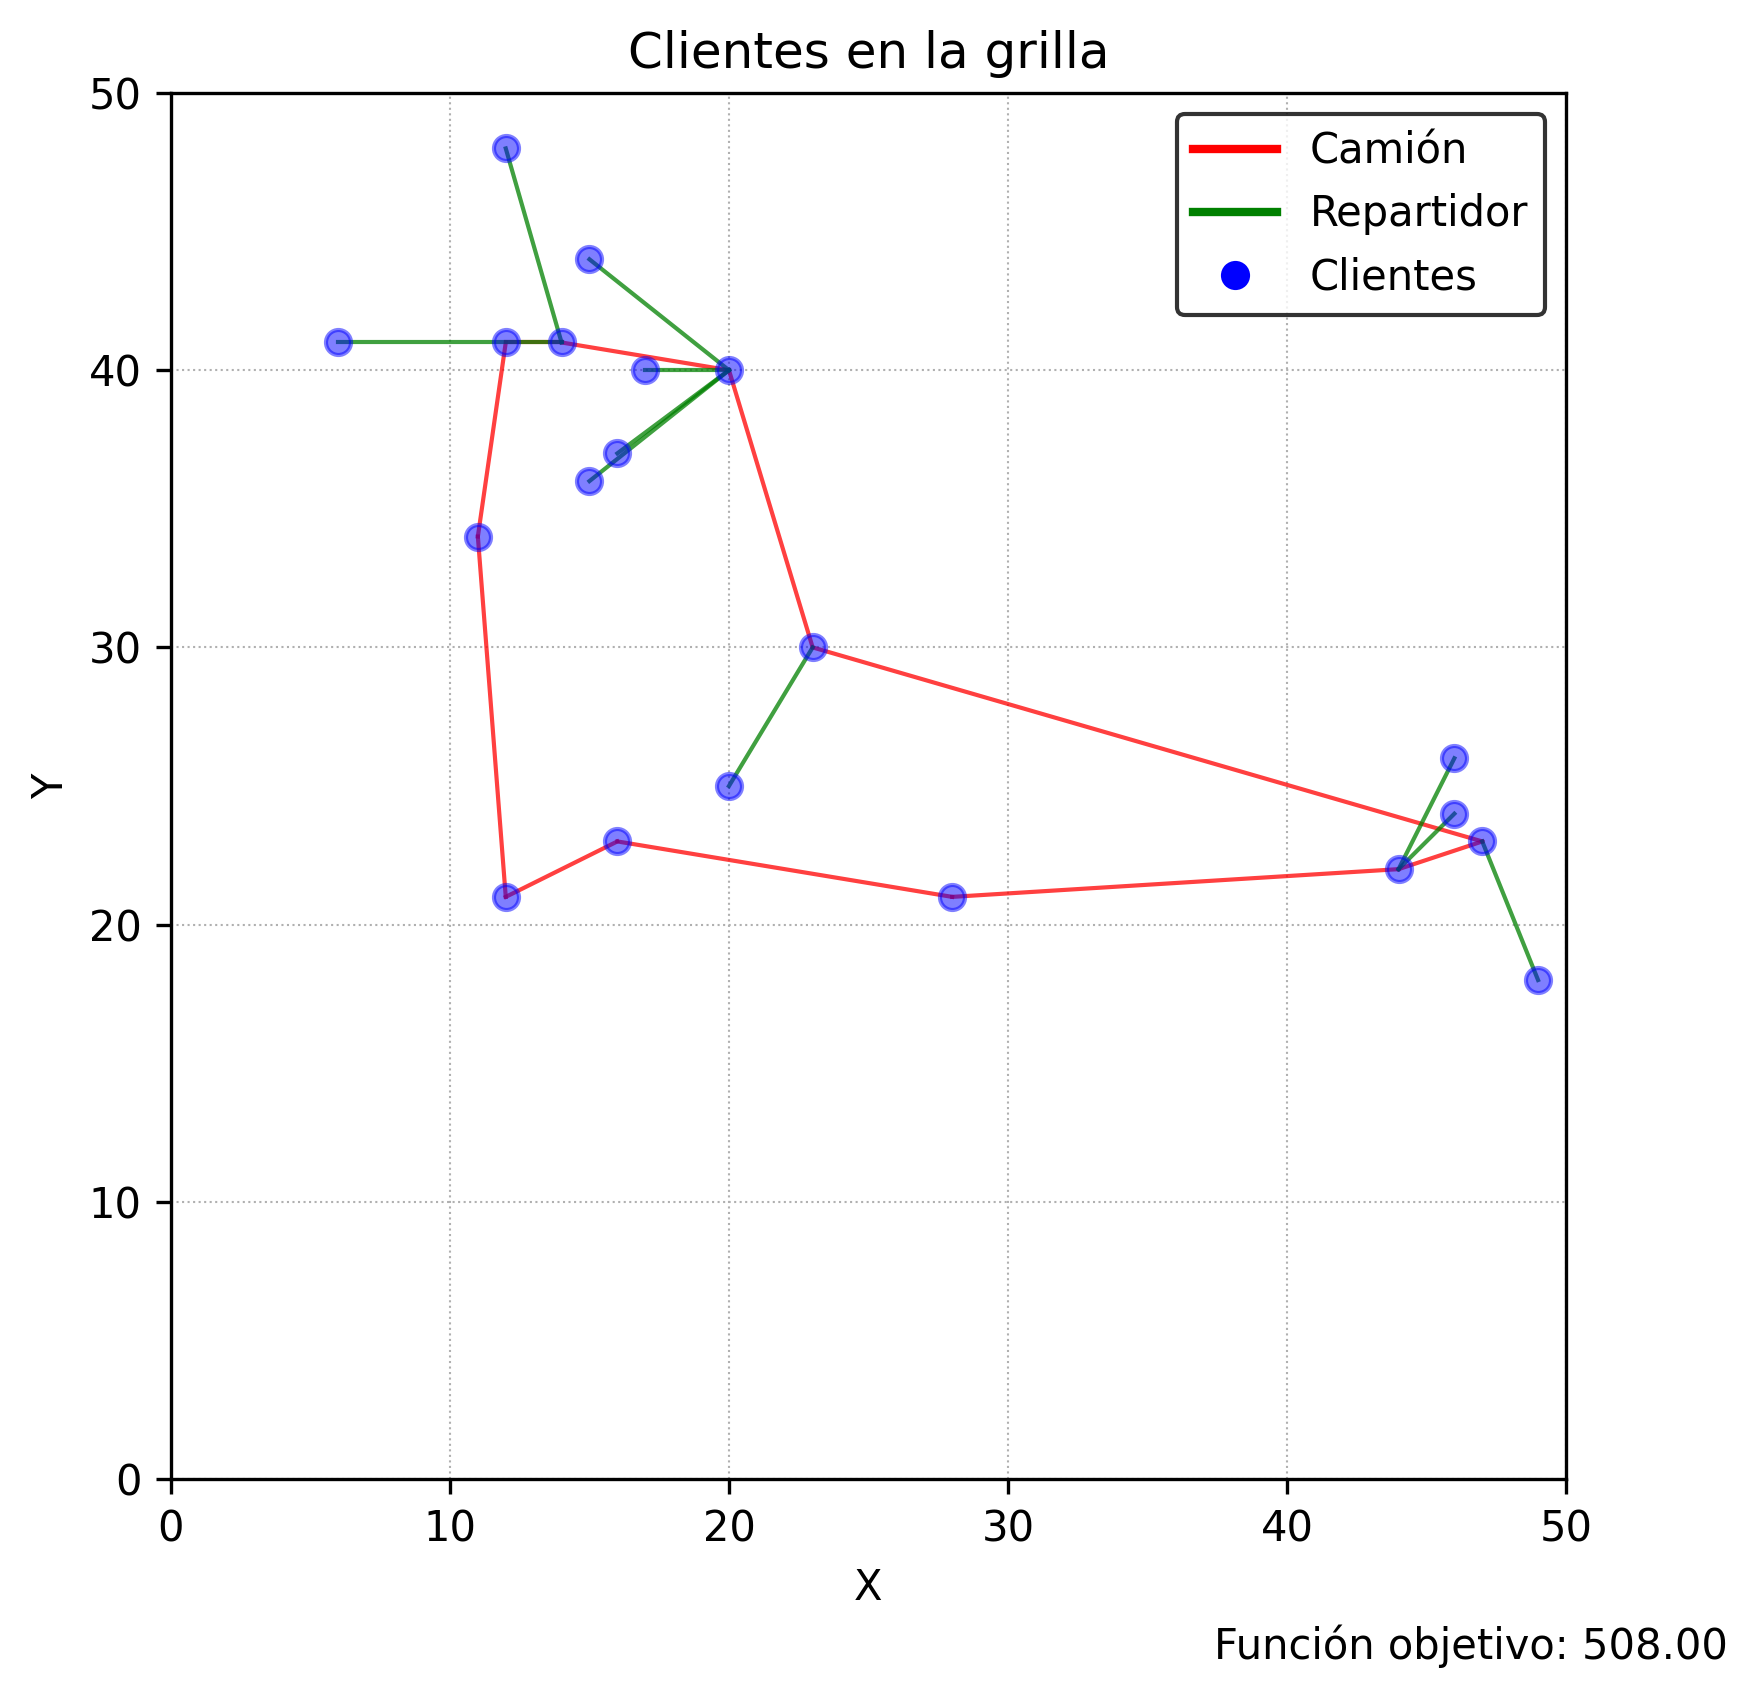
\includegraphics[width=\textwidth]{figuras/plano_clusters_exclusivos_0.png}
		\caption{Metodología con clientes exclusivos (MRE)}
		\label{fig:sub4}
	\end{subfigure}
	
	\caption{Optimización de una misma instancia de \textbf{clusters} con los distintos modelos.}
	\label{fig:compuesta2}
\end{figure}

\subsection{Análisis por metodología e instancia}
Con el fin de relevar la diferencia en costos, generamos 50 instancias uniformemente distribuidas y 32 instancias del tipo cluster, menos cantidad debido a que fueron instancias que requirieron mucho mas tiempo de procesamiento, muy probablemente por que en estas instancias las variables de repartidores juegan un rol crucial para reducir costos. Cada una de las instancias, independientemente del tipo, las evaluamos con las cuatro metodologías distintas. 
En la figura~\ref{fig:barras_costos} se muestran los resultados donde, como era esperable para las instancias con clusters, cualquier metodología con repartidores en general va a tener un menor costo de reparto que la metodología actual. 

\begin{figure}[htbp]
	\centering
	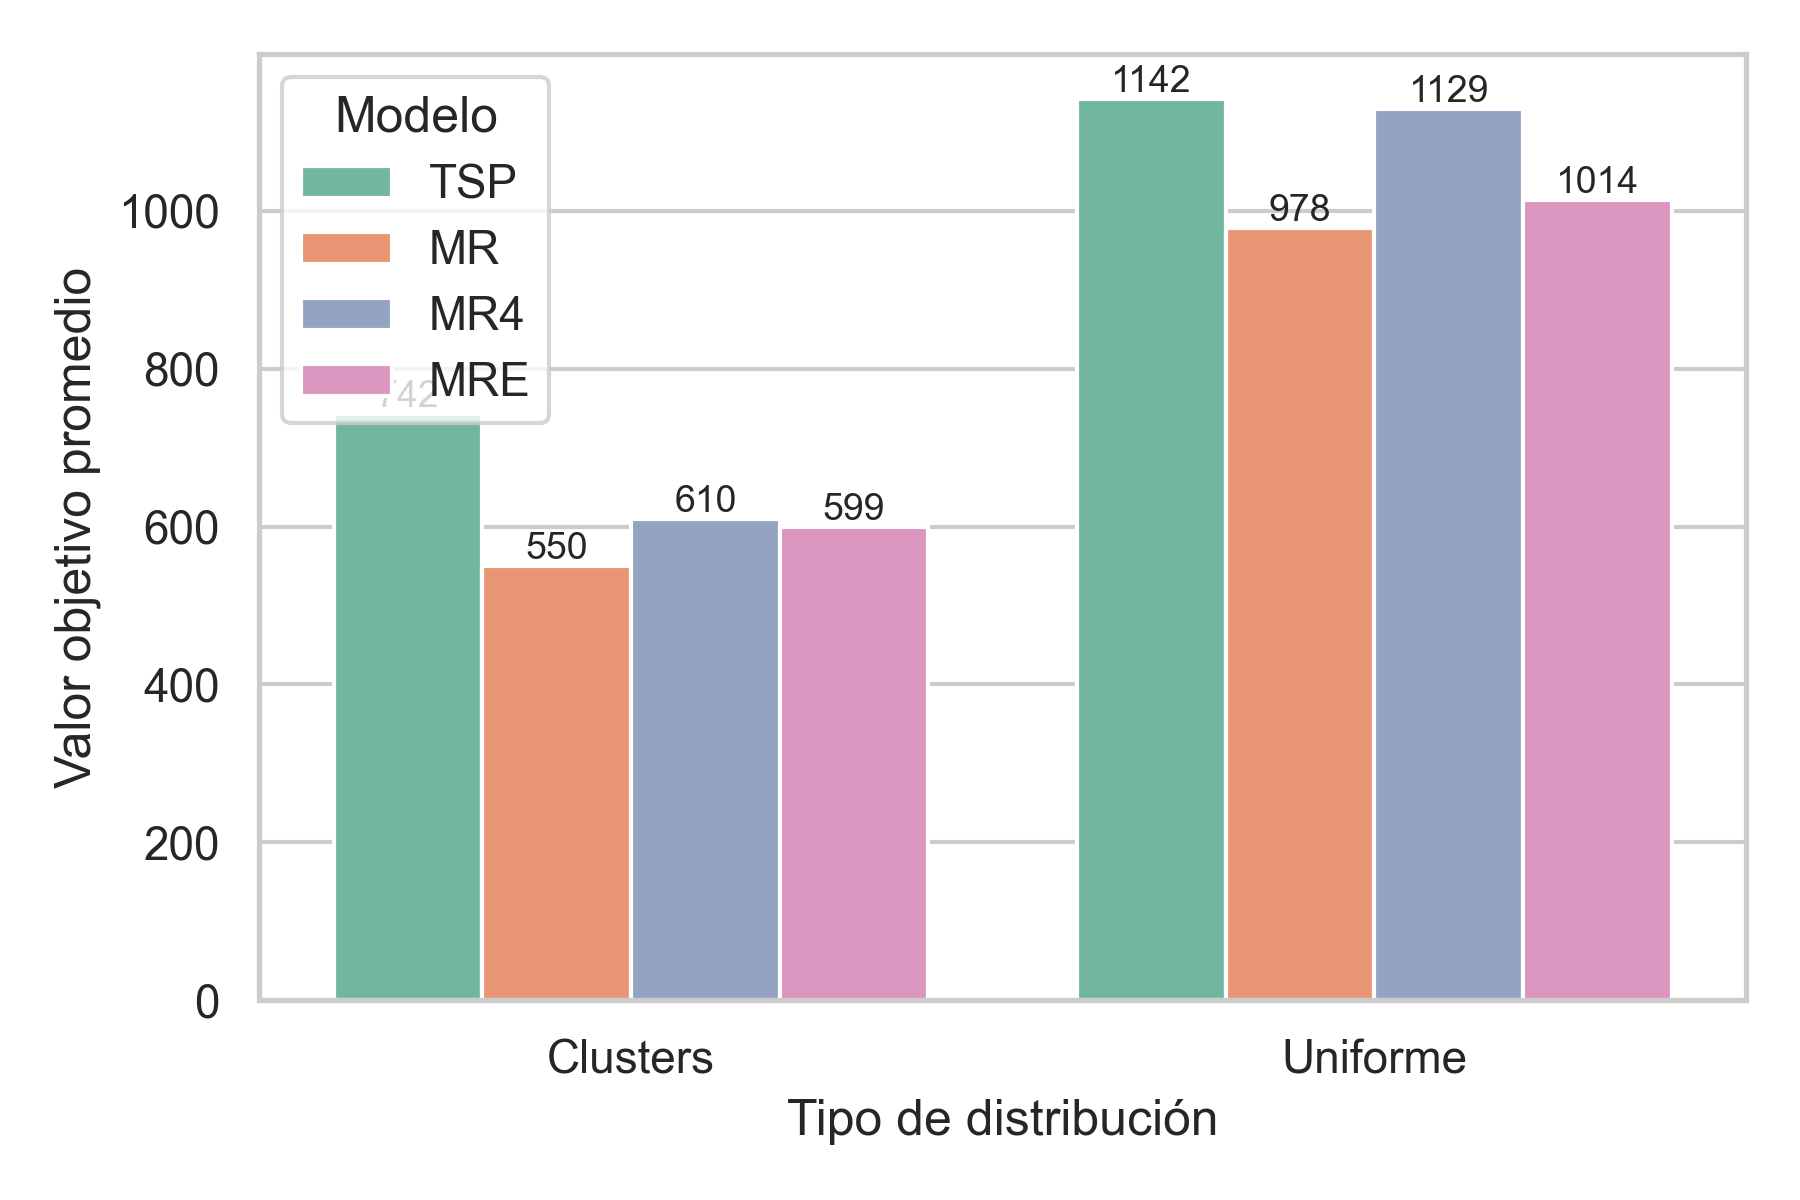
\includegraphics[width=0.7\textwidth]{figuras/barras_costos.png}
	\caption{Gráfico de barras comparando valores objetivos obtenidos}
	\label{fig:barras_costos}
\end{figure}

\clearpage

\section{Tiempos de cómputo CPLEX}

\end{document}
